% !TeX spellcheck = en_US
\documentclass[11pt]{article}

\usepackage{enumitem}
\usepackage{graphicx}
%opening
\title{Advanced Machine Learning - Assignment 4}
\author{Pranav Kasela \\$846965$}
\date{}

\begin{document}

\maketitle

\section*{Introduction}
The dataset consists of images ($150\times150$) with 6 classes: Forest, Mountains, Buildings, Sea, Glacier and Street (Figure \ref{fig:example}). The data is divided in 14034 training samples and 3000 test samples, the training set is splitted into training and validation (80\%-20\%) during the training to test different hyperparameters.
\begin{figure}[!h]
  \centering
  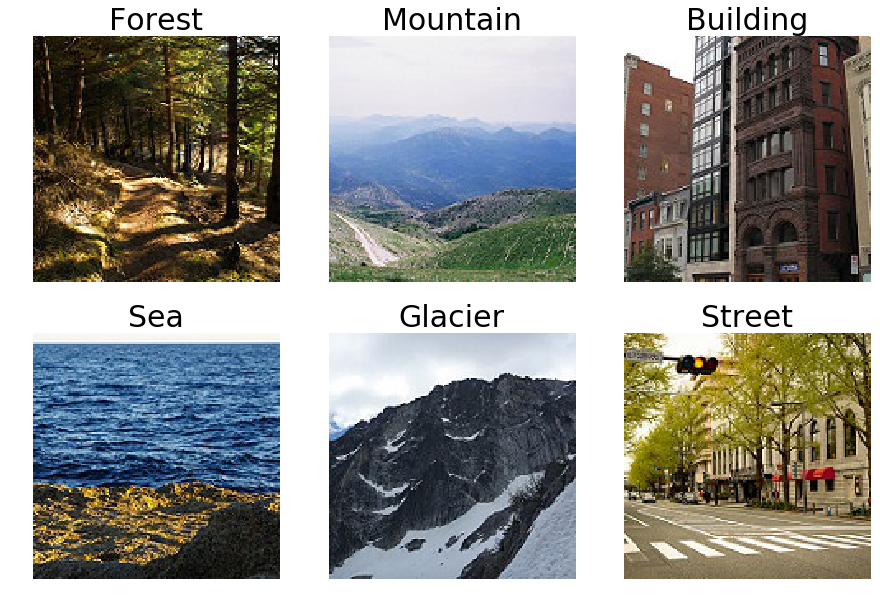
\includegraphics[width=\linewidth, height=6cm]{imgs/samples.png}
  \caption{Example of the 6 classes.}
  \label{fig:example}
\end{figure}

For the assignment the transfer model used is VGG16, the head of the architecture (without the final FC layers) is represented in Figure \ref{fig:VGG16} along with the points where the three cuts are done the features are extracted with a GlobalMaxPooling in all three cuts.
After the feature extraction the best model found is SVM with linear kernel in all three cases.
\begin{figure}[!h]
  \centering
  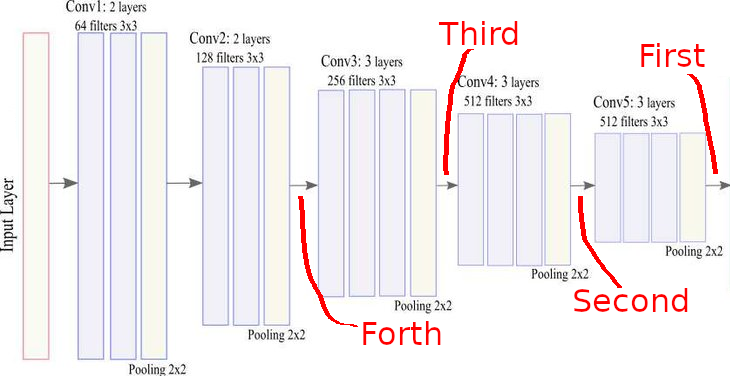
\includegraphics[width=\linewidth, height=5cm]{imgs/VGG16.png}
  \caption{Top of VGG16 Architecture and the cuts for Transfer Learning}
  \label{fig:VGG16}
\end{figure}

\section*{Results}
Both in the First and Second cut the feature extracted are 512, while in the Third cut there are 128 features, these cut are done to see how much the classic machine learning classification models are able to distinguish the images based on the the results obtained by VGG16 pretrained on imagenet.\\
Here are the accuracy results using the Support Vector Classifier with linear kernel, the C coefficient is different in all three cases, only the C with the best performance on validation was chosen:
\begin{center}
  \begin{tabular}{|l|c|c|c|}
    \hline
    & Train & Validation & Test\\
    \hline
    First Cut $(C=0.5)$ & 0.95 & 0.89 & 0.89\\
    \hline
    Second Cut $(C=1)$ & 0.96 & 0.91 & 0.90\\
    \hline
    Third Cut $(C=0.1)$ & 0.85 & 0.83 & 0.83\\
    \hline
  \end{tabular}
\end{center}
The best cut seems to be the Second one, since it obtains similar (better) performance when compared to the First cut, but has to do less calculation to extract the features. In the Third cut the performance got drastically worse, losing about $10\%-11\%$ of accuracy in training and $6\%-8\%$ in test and validation. 

\end{document}
